


\listfiles

\documentclass[	hyperref={pdfpagelabels=false}, xcolor=dvipsnames,
		11pt]{beamer}

% 
\newcommand*{\PTAS}{PTAS}

\newcommand*{\IE}{i.e.}
\newcommand*{\EG}{e.g.}

\newcommand*{\keyword}[1]{\emph{#1}\index{#1}}
% \newcommand*{\comments}[1]{}

\newcommand{\CORR}{\mathrel{\widehat{=}}}

\newcommand*{\SU}[1]{SU(#1)}
% \newcommand*{\Z}[1]{Z(#1)}
\newcommand*{\Z}[1]{\mathbb{Z}_{#1}}

\newcommand*{\DIM}[1]{#1-dimensional}
\newcommand*{\COMMA}{\quad ,}
\newcommand*{\POINT}{\quad .}
\newcommand*{\MEAS}[1]{\mathcal{D}[#1]}


\DeclareMathOperator{\Tr}{tr}
\DeclareMathOperator{\e}{e}

\newcommand*{\tr}[1]{\Tr \ [ \ #1 \ ]}

\newcommand*{\FIG}[1]{Figure~\ref{#1}}
\newcommand*{\FIGs}[2]{Figures~\ref{#1} - \ref{#2}}
\newcommand*{\TAB}[1]{Table~\ref{#1}}
\newcommand*{\SEC}[1]{Section~\ref{#1}}
\newcommand*{\CHAP}[1]{Chapter~\ref{#1}}
\newcommand*{\LIST}[1]{Listing~\ref{#1}}
\newcommand*{\PROC}[1]{Procedure~\ref{#1}}
\newcommand*{\EXP}[1]{\langle #1 \rangle}
\newcommand*{\EQU}[1]{Equation~\eqref{#1}}
\newcommand*{\EQUs}[2]{Equations~(\ref{#1}) - (\ref{#2})}
\newcommand*{\APP}[1]{Appendix~\ref{#1}}

%\newcommand{\tr}[1]{\mbox{tr}~\left[#1]}

\renewcommand\Re{\operatorname{Re}}
\renewcommand\Im{\operatorname{Im}}




\newcommand*{\SYM}[1]{\mathcal{#1}}

\newcommand*{\FIGURE}[1]{\textcolor{blue}{Fig.:}}
% \newcommand*{\FIGURE}[1]{}

%  \newcommand{\testbox}[1]{\framebox{#1}}
\newcommand{\testbox}[1]{#1}

\setlength{\fboxsep}{0.0pt}	%	separation between boxes.
\setlength{\fboxrule}{0.05pt}	%	line width of boxes

\newlength{\plotwidth}
\setlength{\plotwidth}{360pt}

\newlength{\testwidth}
\setlength{\testwidth}{0.25\textwidth}
 
\setlength{\unitlength}{0.95\textwidth}  % measure in textwidths


\newlength{\one}
\setlength{\one}{0.85\textwidth}

\newlength{\onehalf}
\setlength{\onehalf}{0.51\textwidth}

\newlength{\onethird}
\setlength{\onethird}{0.31\textwidth}

\newlength{\twofifth}
\setlength{\twofifth}{0.35\textwidth}


% \def\dblone{\hbox{$1\hskip -1.2pt\vrule depth 0pt height 1.6ex width 0.7pt\vrule depth 0pt height 0.3pt width 0.12em$}}

%     \setbeamerfont{section title}{parent=title}
%     \setbeamercolor{section title}{parent=titlelike}
%     \defbeamertemplate*{section page}{default}[1][]
%     {
%       \centering
%         \begin{beamercolorbox}[sep=8pt,center,#1]{section title}
%           \usebeamerfont{section title}\insertsection\par
%         \end{beamercolorbox}
%     }
%     \newcommand*{\sectionpage}{\usebeamertemplate*{section page}}

\definecolor{arrowred}{RGB}{255,105,105}
\definecolor{arrowblue}{RGB}{105,105,255}
\definecolor{resultgreen}{RGB}{246,255,213}
\definecolor{resultgreenedge}{RGB}{0,128,0}


\AtBeginSection[]{
  \begin{frame}
  \vfill
  \centering
  \begin{beamercolorbox}[sep=8pt,center,shadow=true,rounded=true]{title}
    \usebeamerfont{title}\insertsectionhead\par%
  \end{beamercolorbox}
  \vfill
  \end{frame}
}

% 


\usepackage{etex}			% needed to resolve conflicts between booktabs and tikz
\usepackage{tikz}
\usepackage{verbatim}
\usetikzlibrary{arrows,shapes}

 %\usetheme{boxes}
% \usecolortheme{lily}
 %\usecolortheme{rose}

 \usefonttheme{serif}

\usepackage{lmodern}
 \usepackage{graphicx}
 \usepackage{multirow}				%enables multirow tables

\usepackage{natbib}
\bibpunct{[}{]}{,}

\usepackage{epsfig}
\usepackage{layout}

\usepackage{booktabs}

\setbeamercovered{transparent}
\mode<presentation>





 
\beamertemplatenavigationsymbolsempty %Navigationszeile auf jeder Folie unterdrücken






\usepackage{ae,aecompl}				% fuer besseres pdf empfohlen
%\usepackage{exscale}				% richtige Skalierung der Mathe Formeln. Does not work with tikz




\usepackage[mathcal]{euscript}
\usepackage{amsthm}				% adds theorems and lemmata



\usepackage{dsfont}

% \usepackage{fancyhdr}	


% 
% %******************************************************************************
% %
% % Fancyheaders
% %
% \usepackage{fancyhdr}					% Pagehead
% \pagestyle{fancy}					% meine Kopfzeile
% \fancyhf{}
% % \fancyhead[RO]{\rm \nouppercase  \rightmark \qquad \rm \thepage }
% % \fancyhead[LE]{  \thepage  \qquad \rm \nouppercase  \leftmark }
% \fancyhead[RO]{\nouppercase  \rightmark}
% \fancyhead[LE]{ \nouppercase  \leftmark }
% 
% \fancyfoot[OR]{  \thepage}
% \fancyfoot[EL]{ \thepage }
% 
% % \renewcommand{\headrulewidth}{0.1pt}
% 
% \renewcommand{\chaptermark}[1]{\markboth{\thechapter.\ #1}{}}
% 
% 
% \renewcommand{\sectionmark}[1]{\markright{\thesection.\ #1}}
% 
% 
% \fancypagestyle{plain}{%
% \fancyhf{} % clear all header and footer fields
% \fancyfoot[RO,RE]{\thepage} %RO=right odd, RE=right even
% \renewcommand{\headrulewidth}{0pt}
% \renewcommand{\footrulewidth}{0pt}}
% 
% 
% 
% %
% %******************************************************************************






\usepackage{array}		%for readjusting the hight of lines in tables
% \usepackage{longtable}

\usepackage[german,english]{babel}
\usepackage{hyperref}
\hypersetup{colorlinks=false}
%
\DeclareGraphicsExtensions{.eps, .jpg, .png, .sgv, .jepg}
% \usepackage[subsection]{algorithm}
% \usepackage{algorithmic,algorithmic-fix}
\usepackage{listings}
\lstset{ %
language=C++,                   % the language of the code
basicstyle=\footnotesize,       % the size of the fonts that are used for the code
numbers=left,                   % where to put the line-numbers
numberstyle=\footnotesize,      % the size of the fonts that are used for the line-numbers
stepnumber=1,                   % the step between two line-numbers. If it's 1, each line 
                                % will be numbered
numbersep=5pt,                  % how far the line-numbers are from the code
% showspaces=false,               % show spaces adding particular underscores
% showstringspaces=false,         % underline spaces within strings
showtabs=false,                 % show tabs within strings adding particular underscores
frame=bottomline,                   % adds a frame around the code
% tabsize=2,                      % sets default tabsize to 2 spaces
captionpos=t,                   % sets the caption-position to bottom
% breaklines=false,                % sets automatic line breaking
% breakatwhitespace=false,        % sets if automatic breaks should only happen at whitespace
% title=\lstname,                 % show the filename of files included with \lstinputlisting;
                                % also try caption instead of title
% escapeinside={\%*}{*)},         % if you want to add a comment within your code
% morekeywords={*,...}            % if you want to add more keywords to the set
}


\usepackage{caption}
\DeclareCaptionFont{white}{\color{white}}
\DeclareCaptionFormat{listing}{\colorbox{gray}{\parbox{\textwidth}{#1#2#3}}}
\captionsetup[lstlisting]{format=listing,labelfont=white,textfont=white}











\usepackage{parskip}		%kills the default paragraph indenting and sets /parskip to some useful value automatically



\usepackage{amssymb}
\usepackage{amsmath}
% \usepackage{bbold}
% \usepackage{dsfont}

%Graphics and Videos




%Graphics and Videos

% \usepackage{movie15}






\usepackage{thesisstyle}
\usepackage{thesiscommands}

\logo{
\includegraphics[width=1cm]{./pics/unilogo}}


\title{Preliminaries for Distributed Natural Computing Inspired by the Slime Mold Physarum Polycephalum}
\author{Michael T.\ Dirnberger}
\institute{Max Planck Institute for Informatics}

\date{PhD Defense, 31.07.2017, Saarbr\"ucken\\[2em]}


\begin{document}

\begin{frame}[plain]

\titlepage
\vspace{-1cm}
	    \begin{center}
		
\includegraphics[width=0.3\linewidth]{./pics/mpilogo}
	    \end{center}
\end{frame} 


% \section{Part I: Natural Computing with P.~polycephalum}

% \begin{frame}
%     \frametitle{Natural Computing in a Nutshell} 

% 	\begin{columns}
% 	\begin{column}{5cm}

% 	\begin{overprint}

% 		 \begin{itemize}
% 		   \item<2-> Design of novel nature inspired algorithms.
% 		   \item<3-> Synthesize natural phenomena by using computers.
% 		   \item<4-> Use natural materials to do computations.
% 		 \end{itemize}

% 	\end{overprint}

% 	\end{column}

% 	\begin{column}{5cm}
% 	\begin{overprint}


% 	\testbox{
% 	     \begin{minipage}[t]{5 cm}

% 			\begin{figure}[h]
			 
% 			     \begin{center}
% 			      \testbox{\includegraphics[angle=0,clip=true,width= 1.6\onethird, trim = 0 0 0 0]<1>{./pics/natural_computing.png}}
% 			      \testbox{\includegraphics[angle=0,clip=true,width= 1.6\onethird, trim = 0 0 0 0]<2>{./pics/ants.jpg}}
% 			      \testbox{\includegraphics[angle=0,clip=true,width= 1.75\onethird, trim = 0 0 0 0]<3>{./pics/weeds.jpg}}
% 			      \testbox{\includegraphics[angle=0,clip=true,width= 1\onethird, trim = 0 0 0 0]<4>{./pics/dna.png}}
% 			     \end{center}

% 			\end{figure}
% 	     \end{minipage} }

% 	\testbox{
% 	     \begin{minipage}{5 cm}
% 	      \begin{center}

% 		\tiny{ Image source: Wikipedia CC BY-SA 4.0}
		

% 	      \end{center}
% 	\end{minipage} }

% 	\end{overprint}
% 	\end{column}
% 	\end{columns}

% 	% \vspace{-0.75cm}
% 	\begin{center}
% 	Natural Computing is a highly interdisciplinary field!
% 	\end{center}
% \end{frame}

% \begin{frame}
%     \frametitle{Meet a Magnificent Mold} 

% 	\begin{columns}
% 	\begin{column}{4.6cm}

% 	\begin{overprint}

% 		\begin{block}{\emph{Physarum Polycephalum}:}
% 		  \begin{itemize}
% 		   \item<2> Unicellular organism with many nuclei.
% 		   \item<3> Intricate foraging strategy.
% 		   \item<4> Networks distribute protoplasm.
% 		  \end{itemize}
% 		\end{block}

% 	\end{overprint}

% 	\end{column}

% 	\begin{column}{5cm}
% 	\begin{overprint}

% 	\testbox{
% 	     \begin{minipage}[t]{5 cm}

% 	\begin{figure}[h]
	 
% 	     \begin{center}
% 	      \testbox{\includegraphics[angle=0,clip=true,width= 1.6\onethird, trim = 0 0 0 0]<1>{./pics/tree_of_life.png}}
% 	      \testbox{\includegraphics[angle=0,clip=true,width= 1.6\onethird, trim = 0 0 0 0]<2>{./pics/physarum_forest.jpg}}
% 	      \testbox{\includegraphics[angle=0,clip=true,width= 1.6\onethird, trim = 0 0 0 0]<3>{./pics/physarum_exploring_tree_2.jpg}}
% 	      \testbox{\includegraphics[angle=0,clip=true,width= 1.5\onethird, trim = 0 0 0 0]<4>{./pics/physarum.jpg}}
% 	     \end{center}

% 	\end{figure}
% 	     \end{minipage} }

% 	\testbox{
% 	     \begin{minipage}{5 cm}
% 	      \begin{center}

% 		\tiny{Images courtesy of Prof.~T.~Ueda.}
		

% 	      \end{center}
% 	     \end{minipage} }

% 	\end{overprint}
% 	\end{column}
% 	\end{columns}

% 	\vspace{-1cm}

% 	\centering
% 		\begin{alertblock}{\underline{Key Experiments show:}}
% 			Distributed operation, Minimisation/Maximitation capabilities
% 		\end{alertblock}
% \end{frame}

% \begin{frame}
%     \frametitle{Natural Computing with \P} 

% 	\begin{columns}
% 	\begin{column}{4.6cm}

% 	\begin{overprint}

% 		\begin{block}{Succes stories}
% 		  \begin{itemize}
% 		   \item<1> Positive feedback models
% 		   \item<2> Many particle simulations/cellular automata 
% 		   \item<3> Steering \P using light
% 		  \end{itemize}
% 		\end{block}

% 	\end{overprint}

% 	\end{column}

% 	\begin{column}{5cm}
% 	\begin{overprint}

% 	\testbox{
% 	     \begin{minipage}[t]{5 cm}

% 	\begin{figure}[h]
	 
% 	     \begin{center}
% 	      \testbox{\includegraphics[angle=0,clip=true,width= 1.\onethird, trim = 0 0 0 0]<1>{./pics/shortest_path_model.pdf}}
% 	      \testbox{\includegraphics[angle=0,clip=true,width= 1.\onethird, trim = 0 0 0 0]<2>{./pics/mst_agent.png}}
% 	      \testbox{\includegraphics[angle=0,clip=true,width= 1.\onethird, trim = 0 0 0 0]<3>{./pics/container_states.png}}
% 	     \end{center}

% 	\end{figure}
% 	     \end{minipage} }

% 	\testbox{
% 	     \begin{minipage}{5 cm}
% 	      \begin{center}

% 		\tiny{Images courtesy of Prof.~T.~Ueda.}
		

% 	      \end{center}
% 	     \end{minipage} }

% 	\end{overprint}
% 	\end{column}
% 	\end{columns}

% 	\vspace{-1cm}

% 	\centering
% 		\begin{alertblock}{\underline{Caveat:}}
% 			Distributed nature of \P has not been investigated in the context of Natural Computing.
% 		\end{alertblock}
% \end{frame}

% \begin{frame}
%     \frametitle{Towards distributed Natural Computing with \P} 

%     \begin{block}{Our aim:}
%     	Study the networks formed by \P in order to drive the development of a distributed model.
%     \end{block}

% 	\begin{alertblock}{Our approach:}
% 		\begin{itemize}
% 			\item Obtain a large body of experimenta data
% 			\item Process raw experimental data
% 			\item Analyze network properties
% 			\item Model the dynamics exhibited by \P
% 		\end{itemize}
% 	\end{alertblock}
% \end{frame}

\section{Part II: Studying the networks formed by P.~polycephalum}

% \begin{frame}
%     \frametitle{Experiments} 

% 	\begin{overprint}

% 		\begin{figure}[h]
		 
% 			\begin{center}
% 				\testbox{\includegraphics[angle=0,clip=true,width= \one, trim = 0 0 0 0]<1>{./pics/setup.png}}
% 				\testbox{\includegraphics[angle=0,clip=true,width= \one, trim = 0 0 0 0]<2>{./pics/physarum_sequence_1.JPG}}
% 				\testbox{\includegraphics[angle=0,clip=true,width= \one, trim = 0 0 0 0]<3>{./pics/physarum_sequence_2.JPG}}
% 				\testbox{\includegraphics[angle=0,clip=true,width= \one, trim = 0 0 0 0]<4>{./pics/physarum_sequence_3.JPG}}
% 				\testbox{\includegraphics[angle=0,clip=true,width= \one, trim = 0 0 0 0]<5>{./pics/physarum_sequence_4.JPG}}
% 				\testbox{\includegraphics[angle=0,clip=true,width= \one, trim = 0 0 0 0]<6>{./pics/physarum_sequence_5.JPG}}
% 			\end{center}
% 		\end{figure}  
% 	\end{overprint}
% \end{frame}

\begin{frame}
    \frametitle{Network Extraction From Images} 


	\begin{columns}
	\begin{column}{4cm}

	\begin{overprint}

	  
		\begin{block}{NEFI:}
		  \begin{itemize}
		   \item Input: High quality image of a network
		   \item Output: Graph representation of depicted structure
		  \end{itemize}
		\end{block}


	\end{overprint}

	\end{column}

	\begin{column}{3cm}
	\begin{overprint}


	\testbox{
	     \begin{minipage}[t]{5 cm}

	\begin{figure}[h]
	 
	     
	      \testbox{\includegraphics[angle=0,clip=true,width= 1.2\onethird, trim = 0 0 0 0]{./pics/NEFI_workflow.png}}
	      % \testbox{\includegraphics[angle=0,clip=true,width= 1.6\onethird, trim = 0 0 0 0]<2>{./pics/physarum_forest.jpg}}
	      % \testbox{\includegraphics[angle=0,clip=true,width= 1.6\onethird, trim = 0 0 0 0]<3>{./pics/physarum_exploring_tree_2.jpg}}
	      % \testbox{\includegraphics[angle=0,clip=true,width= 1.5\onethird, trim = 0 0 0 0]<4>{./pics/physarum.jpg}}


	\end{figure}
	     \end{minipage} }

	\end{overprint}
	\end{column}
	\end{columns}

	\vspace{-0.75cm}

		\begin{alertblock}{\underline{Design goals:}}
		\begin{itemize}
		  	\item Combine well-known algorithms from Computer Vision, Image Processing and Graph Theory to obtain a new modlular tool.
		  	\item Make it such that non-experts can use it.
		\end{itemize}
		\end{alertblock}
\end{frame}

\begin{frame}
    \frametitle{Analysis of \P networks} 

	\underline{Dataset:} Ca. 38 time series of graphs. A total of 1998 weighted cubic planar graphs.

	\underline{Goal:} Obtain a catalouge of Obersables that describes various aspects of \P networks.
	
	\begin{block}{\underline{Key components:}}
	 \begin{itemize}
	  \item Distributions of observables and their time development.
	  \item Examples: Edge lenghts/widths, Face area/circumference and various other properties
	 \end{itemize}
	\end{block}
\end{frame}

\begin{frame}
    \frametitle{Robustness of \P networks} 
   
	\begin{figure}[h]
	     \begin{center}
	      \testbox{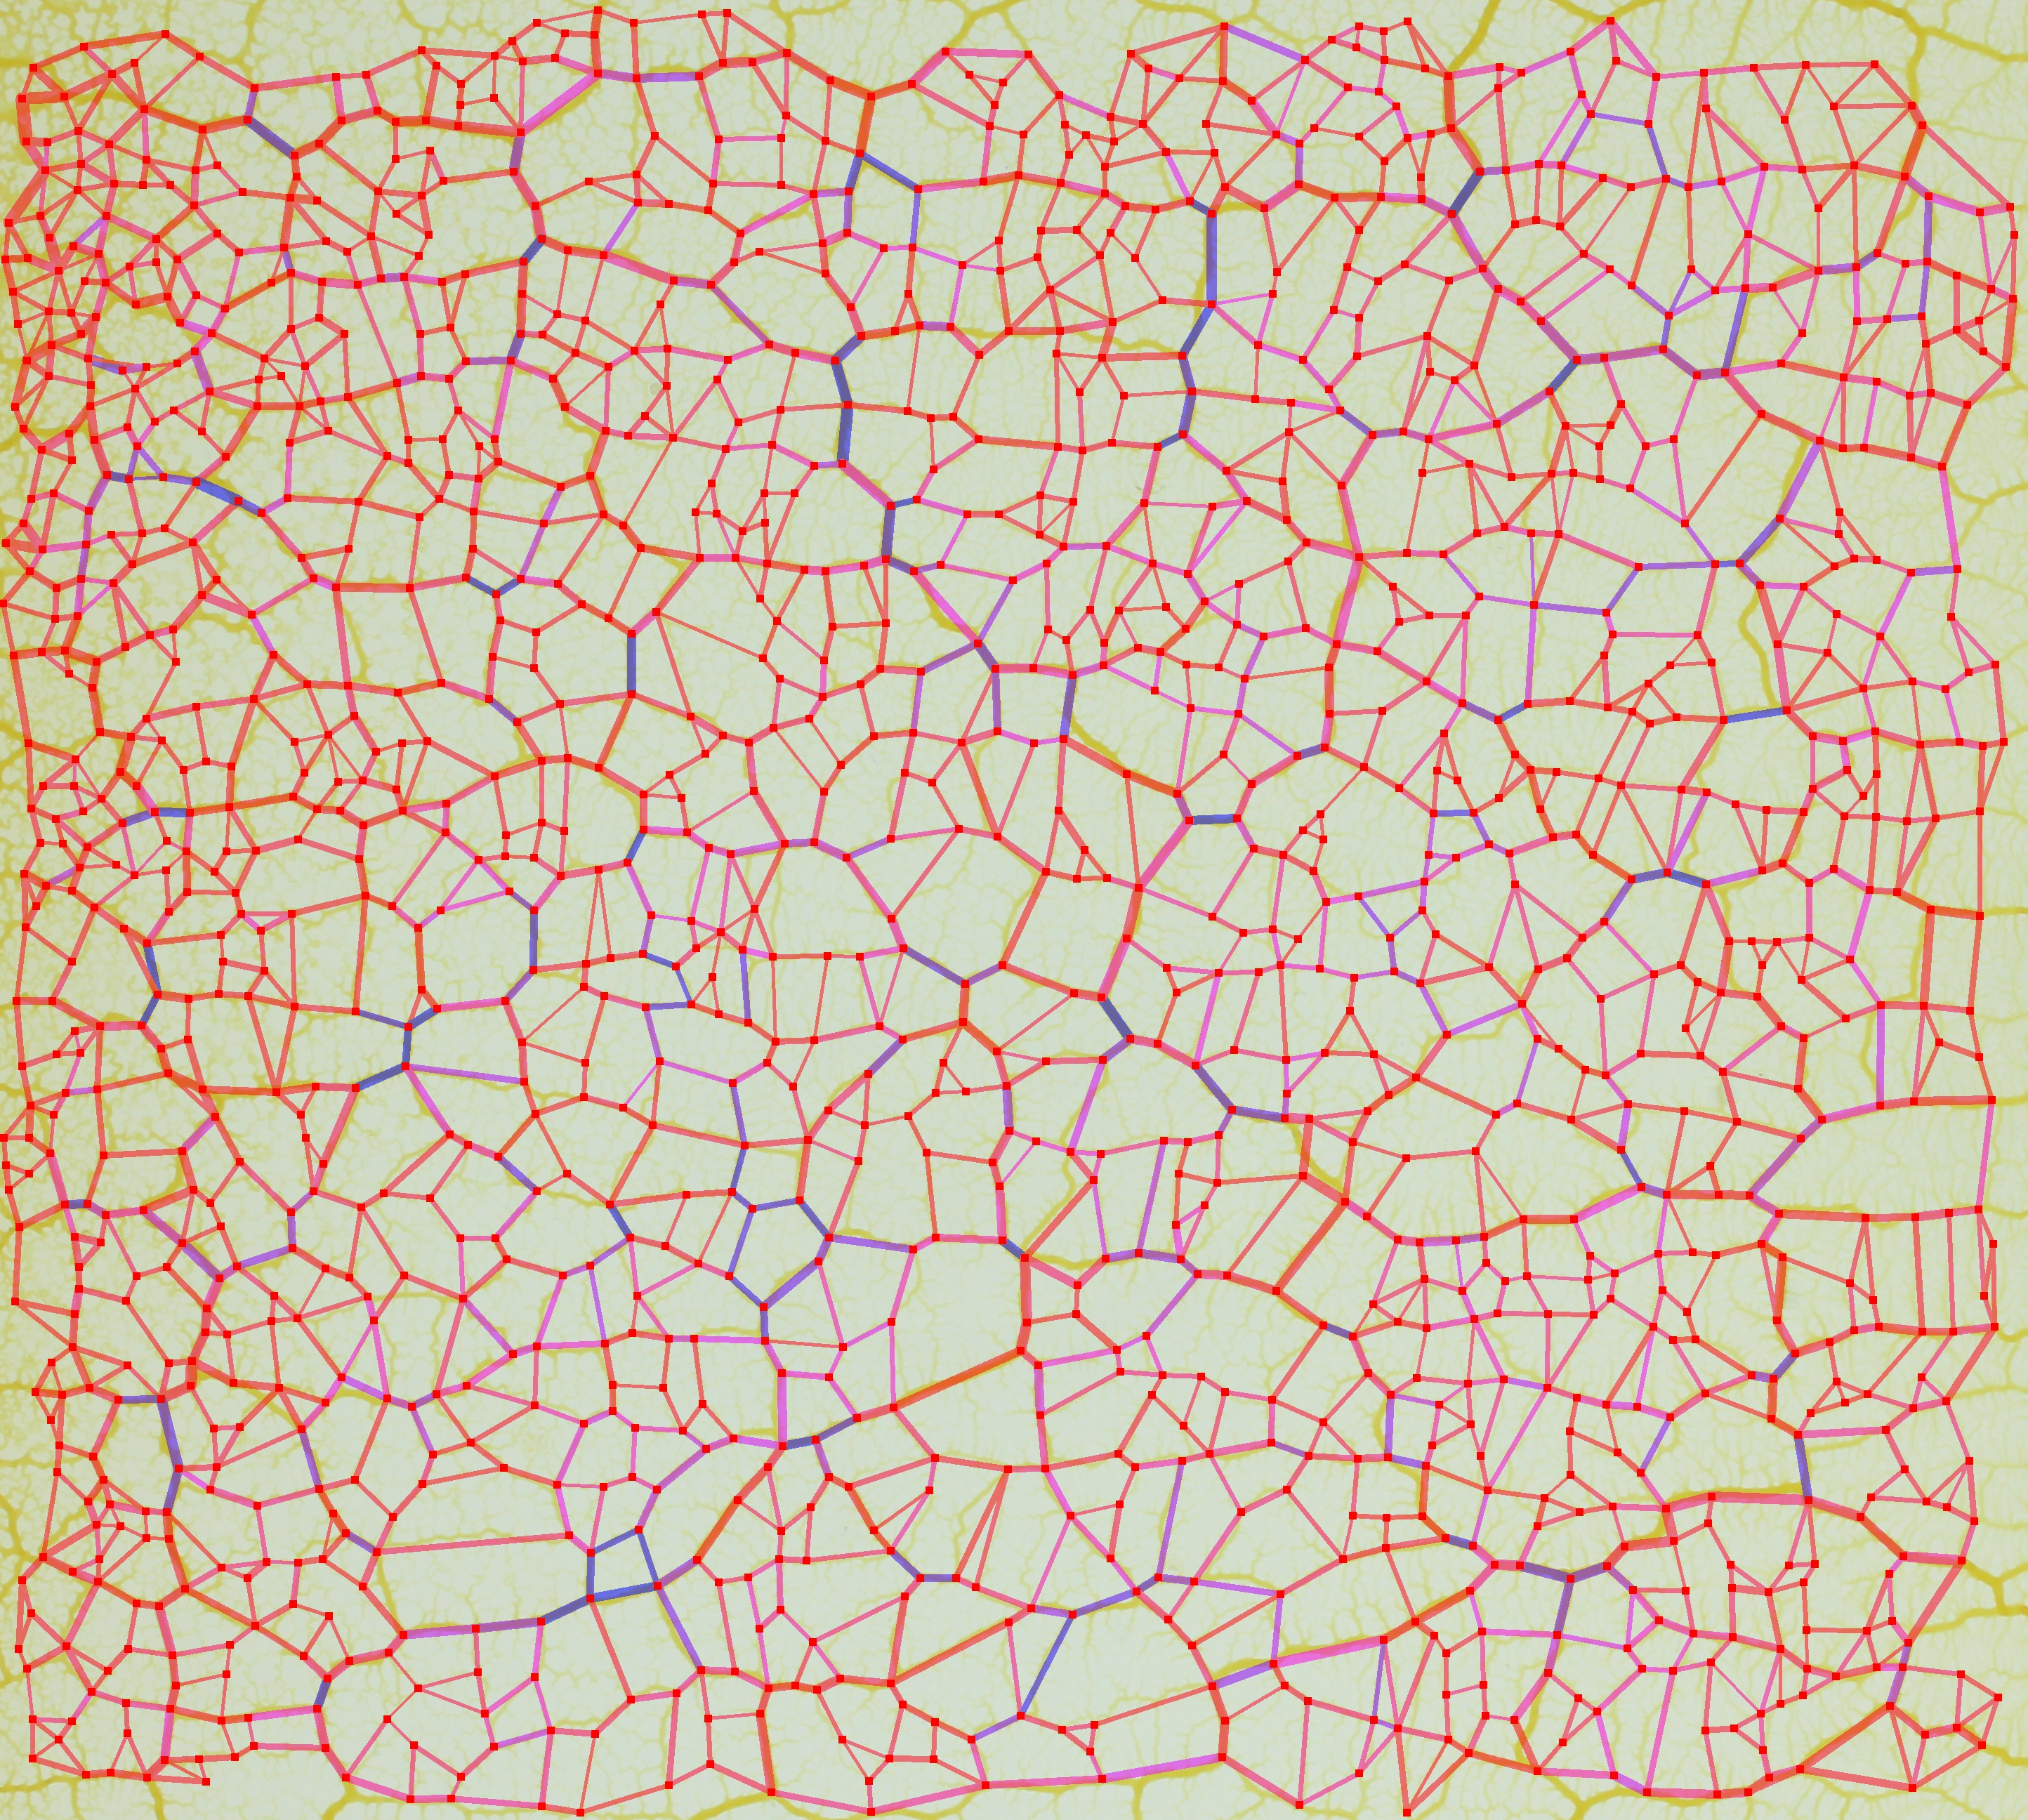
\includegraphics[angle=0,clip=true,width= 0.8\linewidth, trim = 0 0 0 0]{./pics/persistence_heat.jpg}}
	     \end{center}
	\end{figure}
\end{frame}

\begin{frame}
    \frametitle{Robustness of \P networks} 
   
	\begin{figure}[h]
	     \begin{center}
	      \testbox{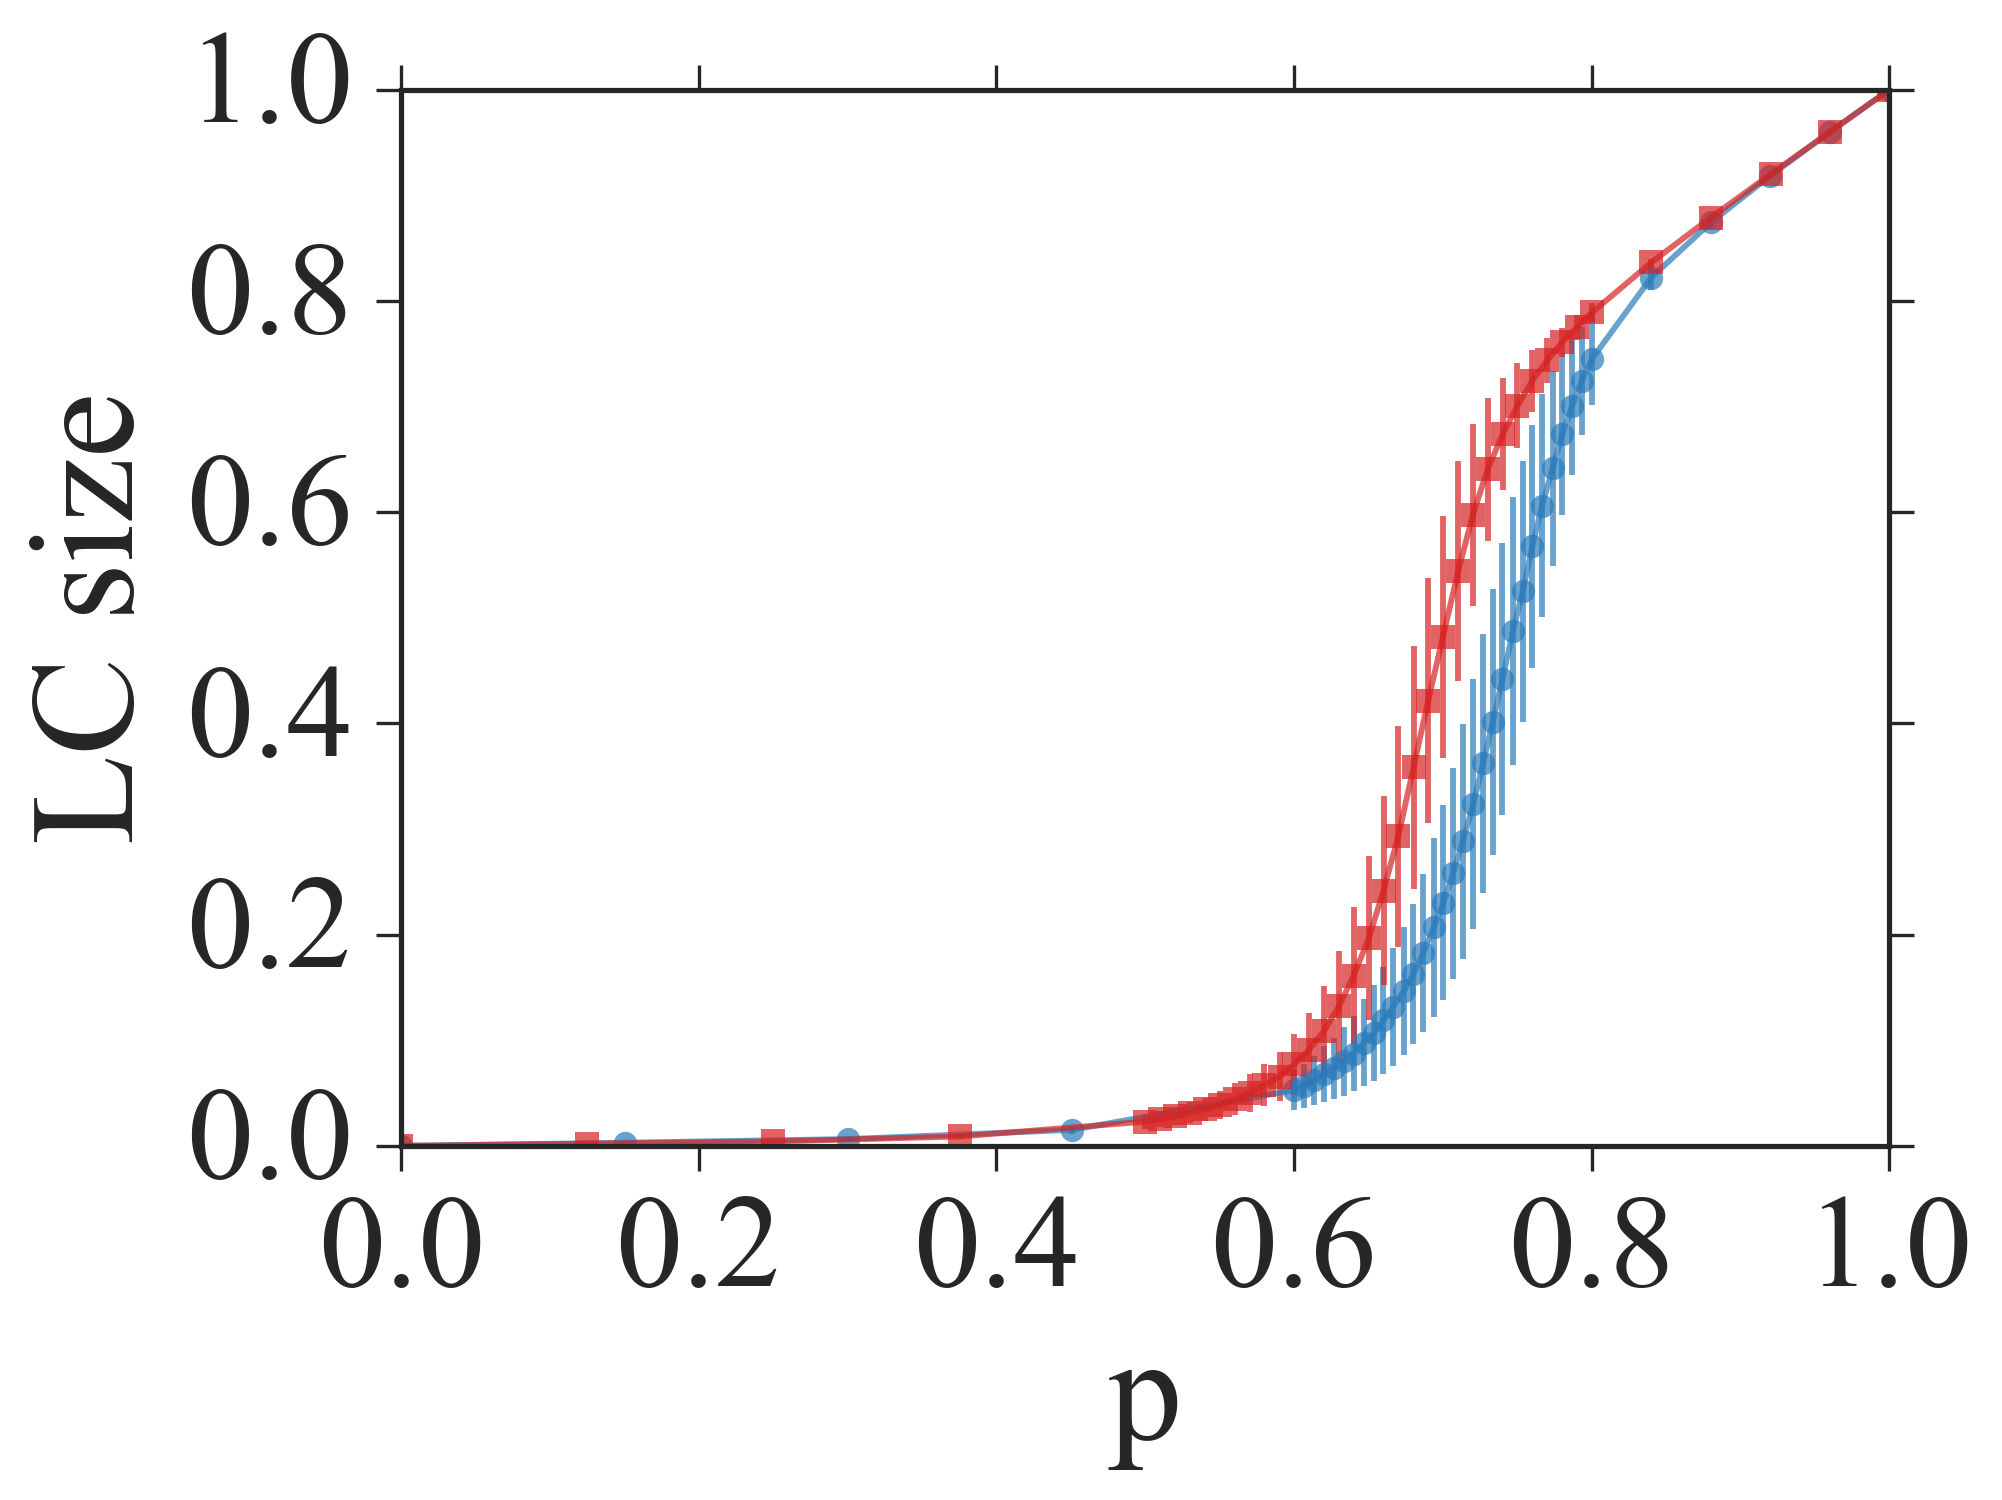
\includegraphics[angle=0,clip=true,width= 0.5\linewidth, trim = 0 0 0 0]{./pics/random_attack_largest_component_motion22.png}}
	      \testbox{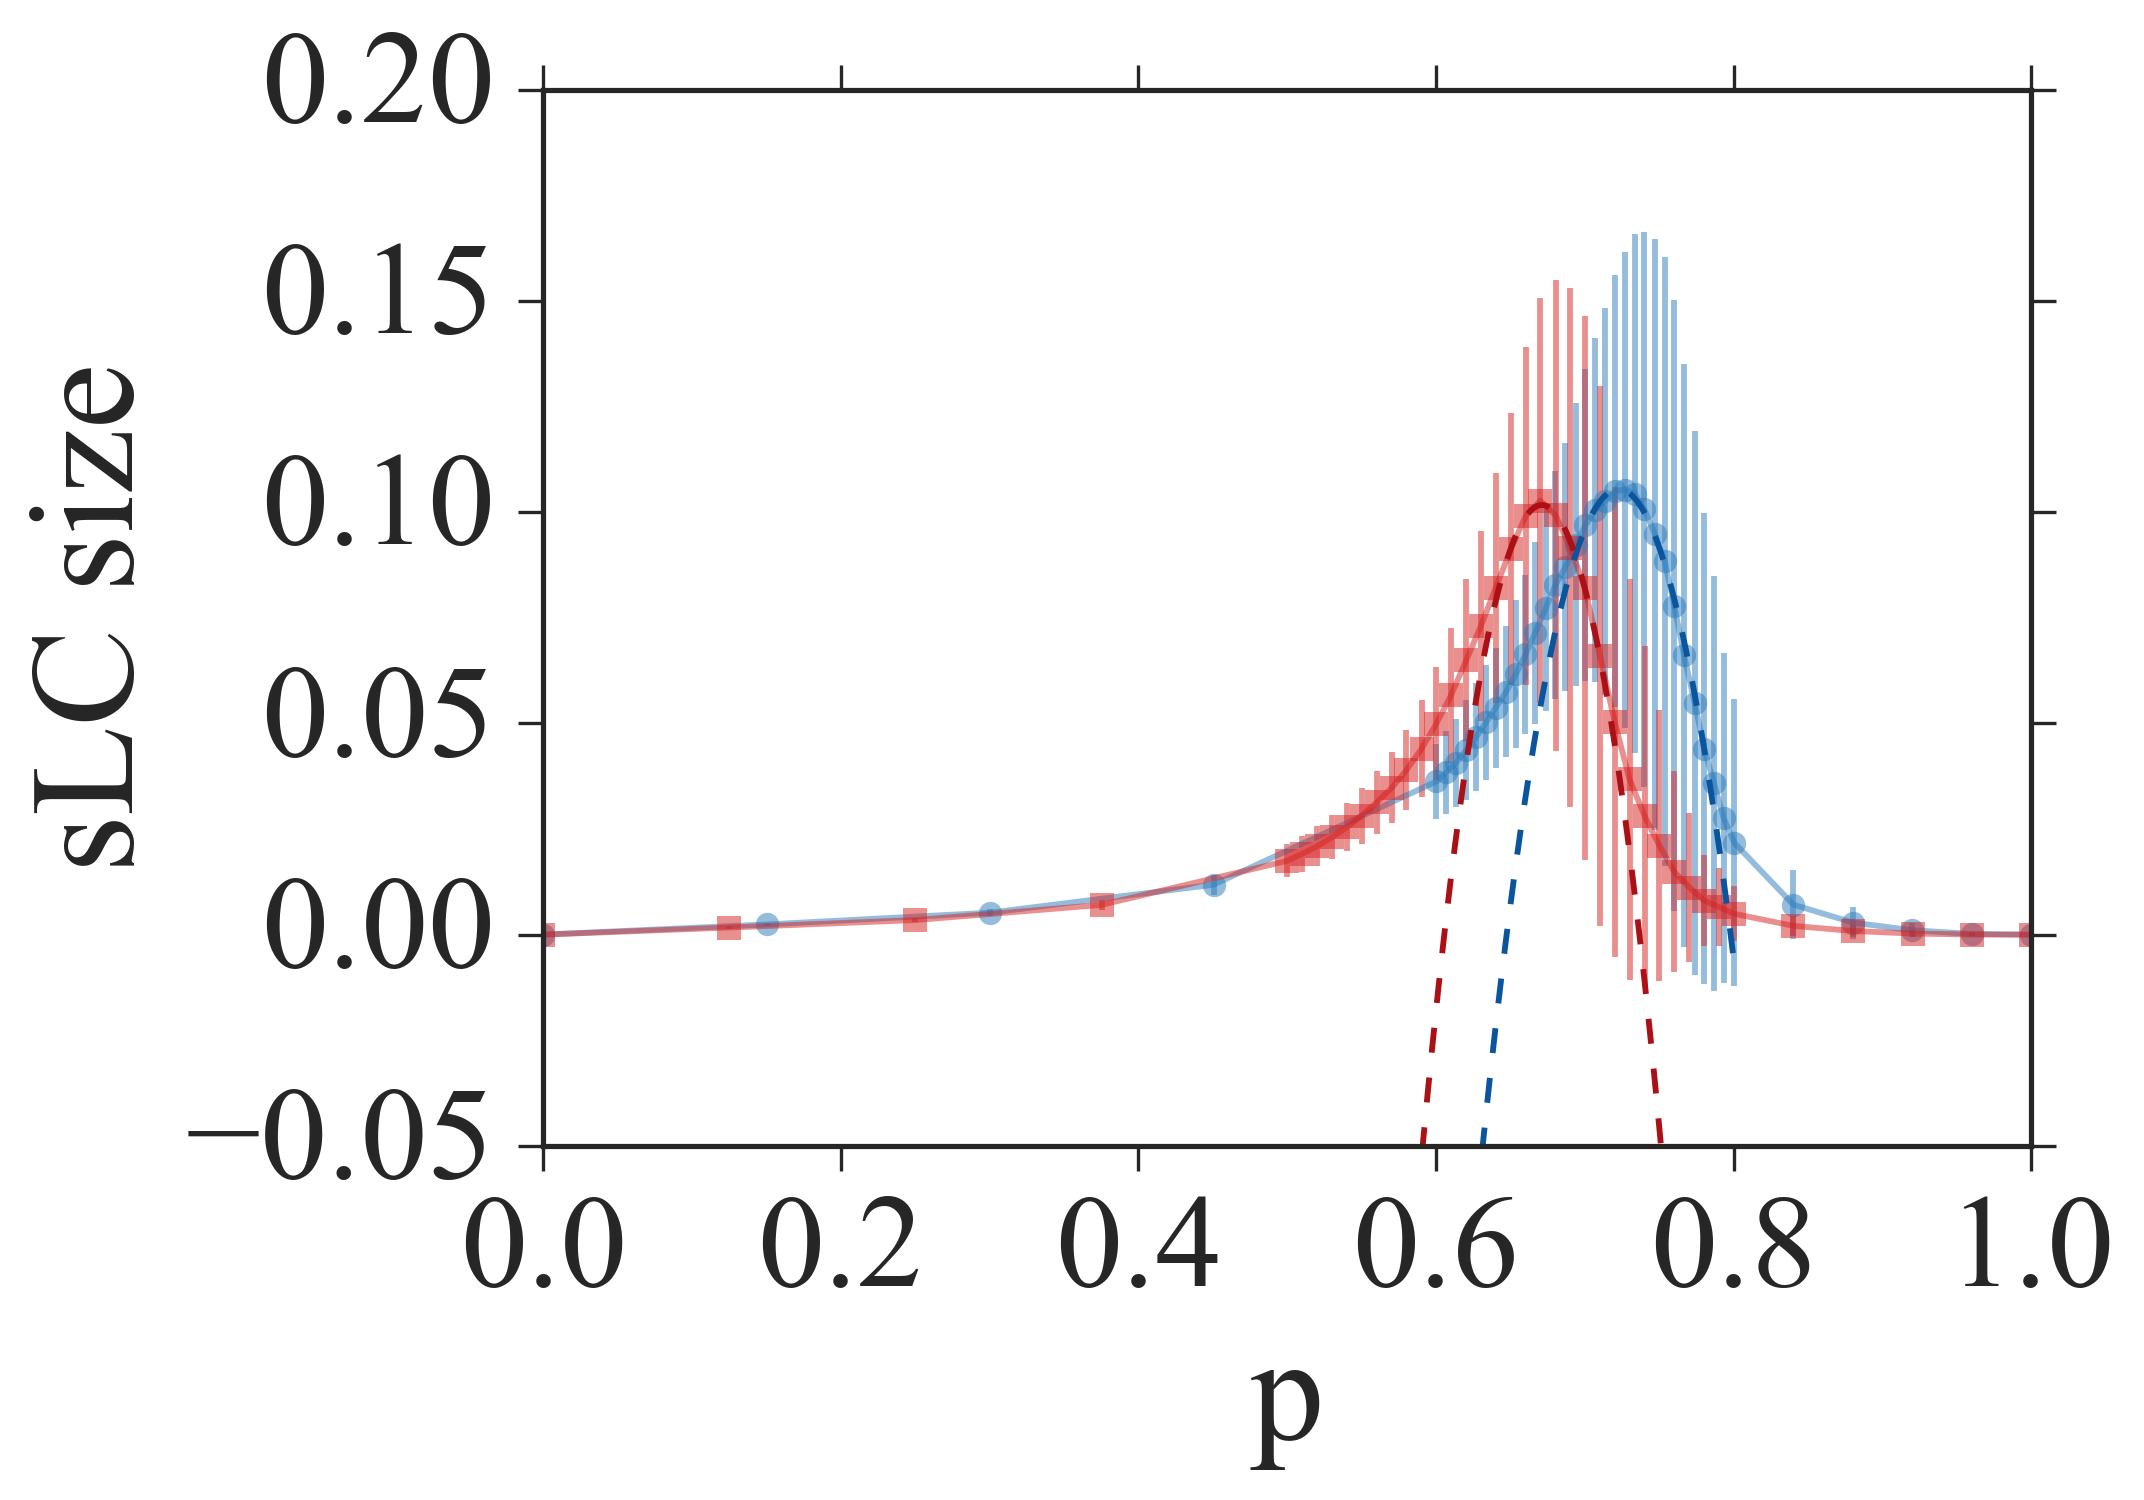
\includegraphics[angle=0,clip=true,width= 0.5\linewidth, trim = 0 0 0 0]{./pics/random_attack_second_largest_component_fit_motion22.png}}
	     \end{center}
	\end{figure}
\end{frame}


\begin{frame}
    \frametitle{SMGR: Sharing is caring} 


	\begin{columns}
	\begin{column}{4cm}

	\begin{overprint}

	  
		\begin{block}{Slime Mold Graph Repository:}
		  \begin{itemize}
		   \item Contains raw experimental data, graphs and useful tools
		   \item Facilitates exchange and reuse of data
		   \item Makes data available to everyone
		  \end{itemize}
		\end{block}


	\end{overprint}

	\end{column}

	\begin{column}{3cm}
	\begin{overprint}


	\testbox{
	     \begin{minipage}[t]{5 cm}

	\begin{figure}[h]
	 
	     
	      \testbox{\includegraphics[angle=0,clip=true,width= 1.2\onethird, trim = 0 0 0 0]{./pics/NEFI_workflow.png}}
	      % \testbox{\includegraphics[angle=0,clip=true,width= 1.6\onethird, trim = 0 0 0 0]<2>{./pics/physarum_forest.jpg}}
	      % \testbox{\includegraphics[angle=0,clip=true,width= 1.6\onethird, trim = 0 0 0 0]<3>{./pics/physarum_exploring_tree_2.jpg}}
	      % \testbox{\includegraphics[angle=0,clip=true,width= 1.5\onethird, trim = 0 0 0 0]<4>{./pics/physarum.jpg}}


	\end{figure}
	     \end{minipage} }

	\end{overprint}
	\end{column}
	\end{columns}

	\vspace{-0.75cm}

		\begin{alertblock}{\underline{Design goals:}}
		\begin{itemize}
		  	\item Combine well-known algorithms from Computer Vision, Image Processing and Graph Theory to obtain a new modlular tool.
		  	\item Make it such that non-experts can use it.
		\end{itemize}
		\end{alertblock}
\end{frame}


% \section{Part III: A distributed model of P.~polycephalum} 

\end{document}
                                       
